\documentclass{article}
\usepackage{amsmath}
\usepackage{hyperref}
\usepackage{amsfonts}
\usepackage{bookmark}
\usepackage{float} 
\usepackage{graphicx}
\usepackage{makeidx}
\usepackage[letterpaper, total={7.5in, 10in}]{geometry}


\makeindex
\begin{document}
\title{Test 1 Prep \\
    \large{Semester 2}}
\author{Elias Xu}
\date{\today}
\maketitle

\setlength{\parindent}{0pt}

\section{Introduction}

Here are Multi Notes to prepare for the first test

\section{Double Integrals}

Double integrals are integrals that represent the volumes under a surface, rather than \textbf{Definite Integrals}, which compute the area under a curve.

\subsection{Definite Integrals Recap}

\begin{figure}[H]
    \centering
    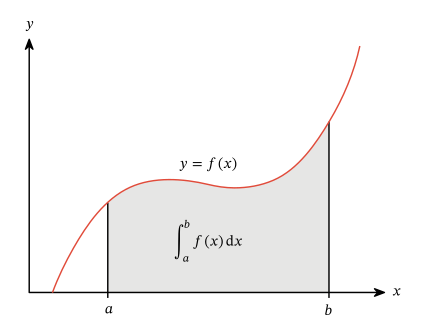
\includegraphics[width=0.2\textwidth]{images/DefiniteIntegralExample.png}
    \caption{Example of a definite Integral}
\end{figure}


Integrals are limits of a Riemann sum, which can be represented by the following equation:
$$\int_{a}^{b} f(x)\delta x = f(x_1)\Delta x_1 + f(x_2) \Delta x_2 + ... = \lim_{n \to \infty} \sum_{i = 1}^{n} f(x_i) \Delta x_i \text{ ,where } \max \Delta x_i \to 0$$

\subsection{Applying Definite Integrals to double integrals}

\begin{figure}[H]
    \centering
    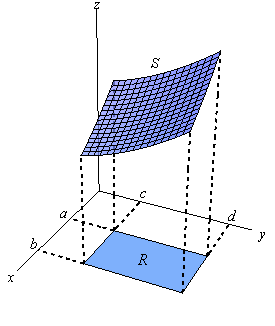
\includegraphics[width=0.2\textwidth]{images/DoubleIntegralsExample.png}
    \caption{Example of a double Integral}
\end{figure}

Given that we have to find the area underneath the curve of a function $z = f(x,y)$, we will need to find \textbf{volume}, not area.\\
We're going to define the rectangle area by:
$$R = \lbrace (x, y) | a \le x \le b , c \le y \le d \rbrace = [a,b] \times [c, d] \text{ (Cartesian Product)}$$ \\
And thus we can define a solid $S$ using the equation:
$$S = \lbrace  (x, y, z) | (x, y) \in \mathbb{R}, 0 \le z \le f(x, y) \rbrace$$ \\
If one is to use equal subintervals to calculate, then you can use a double Riemann sum, with the area of a rectangle equal to $\Delta x \times \Delta y \times f(x,y)$.
You can represent that sum, with
$$\lim_{m, n \to \infty}\sum_{j=1}^{m} \sum_{i=1}^{n} f(x_i^*, y_i^*)\Delta A$$ \\
(\textbf{NOTE} the *'s mean that the values are at a specific point) Where m and n represent the number if subintervals. \\
Double Riemann sums give volume, which when "limited" simplifies to
$$\iint_{R} f(x, y) \delta A = \iint_{[a, b] \times [c, d]} f(x,y) \delta A$$

\subsection{Notes}


\begin{enumerate}
    \item If $f(x, y) \ge 0 \text{ and } f(x, y) \in \mathbb{R}$ then $\iint_{R} f(x, yA) = $ is the volume of the solid bounded by x, y, and the surface
    \item $\delta A = \delta x \delta y \text{ or } \delta y \delta x$. Order will impact evaluation but not result.
    \item If $f(x, y)$ is continious in  $R$, then the double integral exists. (\textbf{NOTE}: You can get away with some discontinuity, such as with steps and the like, but not with stuff like infinite behavior)
\end{enumerate}


\section{Evaluating Double Integrals}

\subsection{Riemann Sums}

\begin{figure}[H]
    \centering
    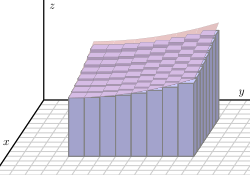
\includegraphics[width=0.2\textwidth]{images/RiemannSumsDoubleIntegralsExample.png}
    \caption{Riemann Sums over Double Integrals}
\end{figure}

Just as with definite integrals, you can use Riemann-esque sums to estimate the area underneath a curve. \\  ~ \\
\textbf{Example Question}: Estimate $\iint_{R} 3x-y^2 \delta A$, where $R = [0,2] \times [0,2]$ using a double Riemann sum using the midpoint  of each rectangle, with $m, n = 2$.\\
To solve, create a grid of a rectangle, and calculate $f(x^*, y^*)$, and multiply that for each rectangle by the $\Delta x$ and $\Delta y$.

\begin{figure}[H]
    \centering
    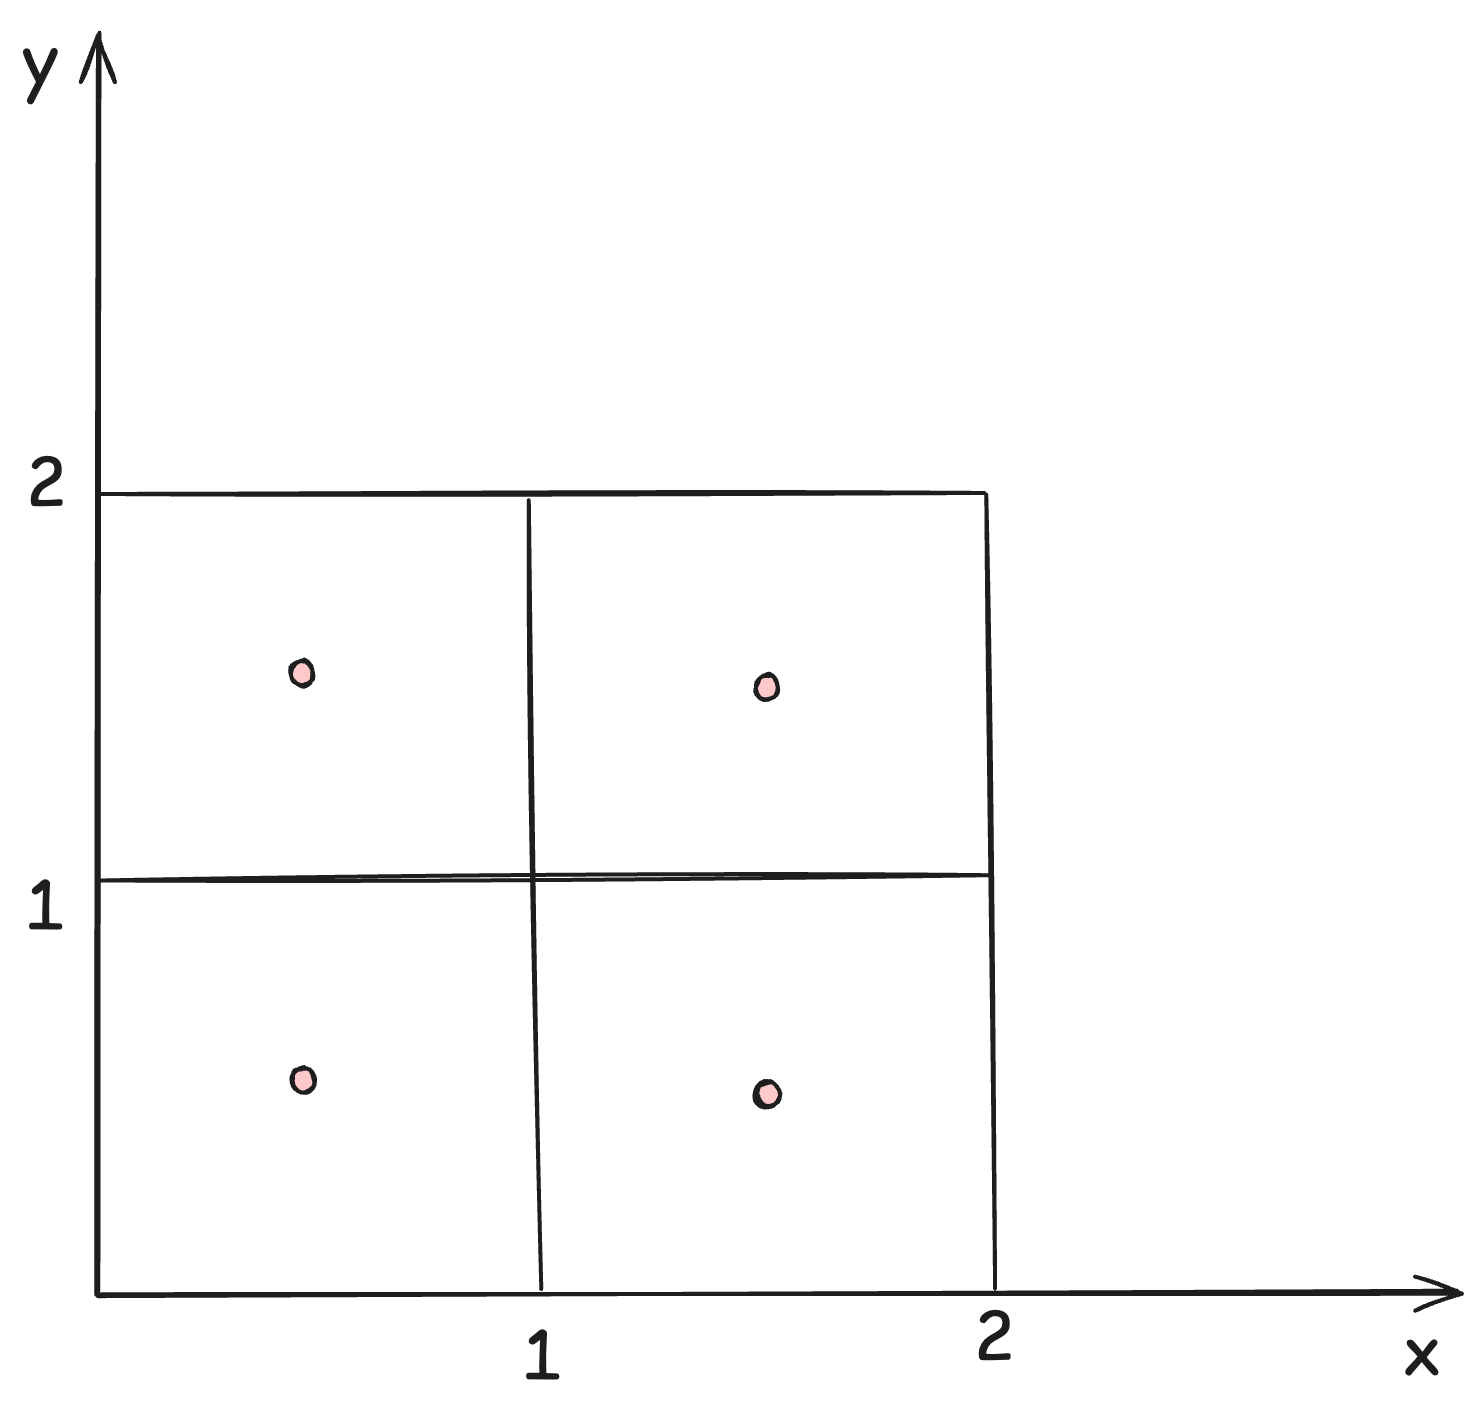
\includegraphics[width=0.2\textwidth]{images/ExampleRectangle.png}
    \caption{Example rectangle, with the points showing the $f(x^*, y^*)$ that is needed to be calculated}
\end{figure}

Once you have the graph, actually solving is relatively straightfoward: $$A \approx f(0.5, 0.5)  \Delta x  \Delta y + f(1.5, 0.5)  \Delta x  \Delta y + f(0.5, 1.5)  \Delta x  \Delta y + f(1.5, 1.5)  \Delta x  \Delta y $$
$$= 1.25 \times 1 \times 1 -0.75 \times 1 \times 1 + 4.25 \times 1 \times 1 + 2.25 \times 1 \times 1 = \boxed{7}$$

There are other ways such a question can be phrased, but the formula/idea should be similar.


\subsection{Fubini's Theorem and Evaluating Double Integrals}

Evaluating double integrals is like counting up loafs of bread, and Fubini's theorem says that no matter how one slices, you'll get the same amount of bread. Y will have to take the slices (integrals over the contours) of either x or y, getting a area function given the other variable, and then integrate that or its range. \\ ~ \\
Thus, Fubini's theorem states that if $f(x, y)$ is continious on $[a, b] \times [c, d]$ then $\iint_{R} f(x, y) \delta A$ equals:
\begin{align*}
    V = \int_{a}^{b} B(x) \delta x = \int_{a}^{b} \left[ \int_{c}^{d} f(x,y) \delta y \right] \delta x  &  & B(x) = \int_{c}^{d} f(x, y) \delta x \\
    V = \int_{c}^{d} A(y) \delta y = \int_{c}^{d} \left[ \int_{a}^{b} f(x, y) \delta x \right] \delta y &  & A(y) = \int_{a}^{b} f(x, y) \delta y
\end{align*}


\section {The Very Nice Theorem}

Interesting way to evauate integrals that can be separated into individual components. 
$$\text{If } f(x, y) = g(x)h(y) \text{ and R} = [a, b] \times [c, d] \text{, then} \\ \iint_{R} f(x, y) \delta A = \int_{a}^{b} g(x) \delta x \int_{c}^{d} h(y) \delta y $$

\section{Double Integral Properties (over Rectangles)}

\begin{itemize}
    \item  $\iint_{R} (f + g) \delta A = \iint_{R} f \delta A + \iint_{R} g \delta A$
    \item $\iint_{R} cf(x,y) \delta A = c \iint_{R} f(x, y) \delta A$
    \item If $f(x, y) \ge g(x, y)$, then $\iint_{R} f(x, y) \delta A \ge \iint_{R} g(x, y)$. (i.e. integrals preserve inequalities)
\end{itemize}

\section{Evaluating Double Integrals over Non-Rectangular Boundaries}

A big idea relating to evaluating double integrals over non-rectangular boundaries is how to find a bound, because it's more interesting/difficult to do so with these odd bounds. Thus we need to differential between type 1, type 2, and non-typal shapes.

\subsection{Type 1 Shapes vs Type 2 Shapes}

\textbf{Type 1 Shapes}\\
Type one shapes have a $x \in \lbrack a, b \rbrack$ as boundaries, and are defined by two $y = g(x)$ functions. 
\begin{figure}[H]
    \centering
    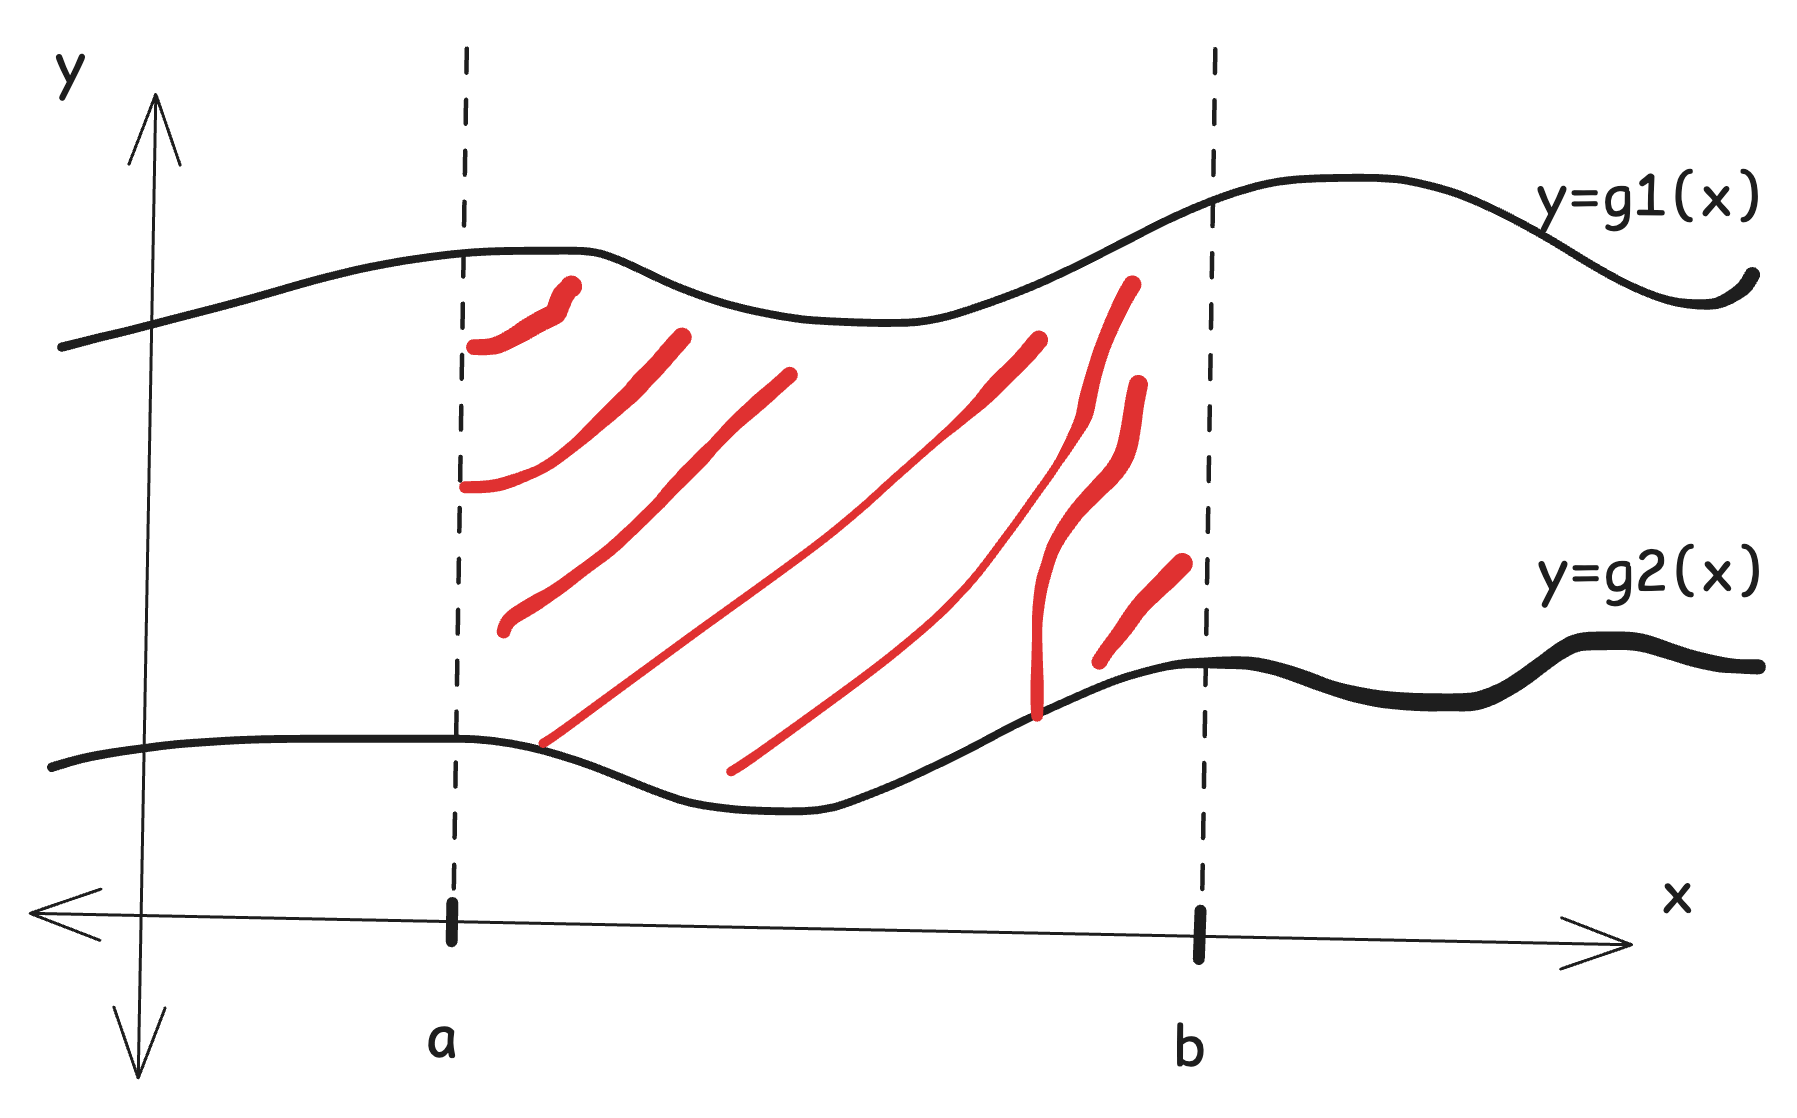
\includegraphics[width=0.5\textwidth]{images/Type1Example.png}
    \caption{Example of a Type 1 bound}
\end{figure}
\textbf{Type 2 Shapes} 

\begin{figure}[H]
    \centering
    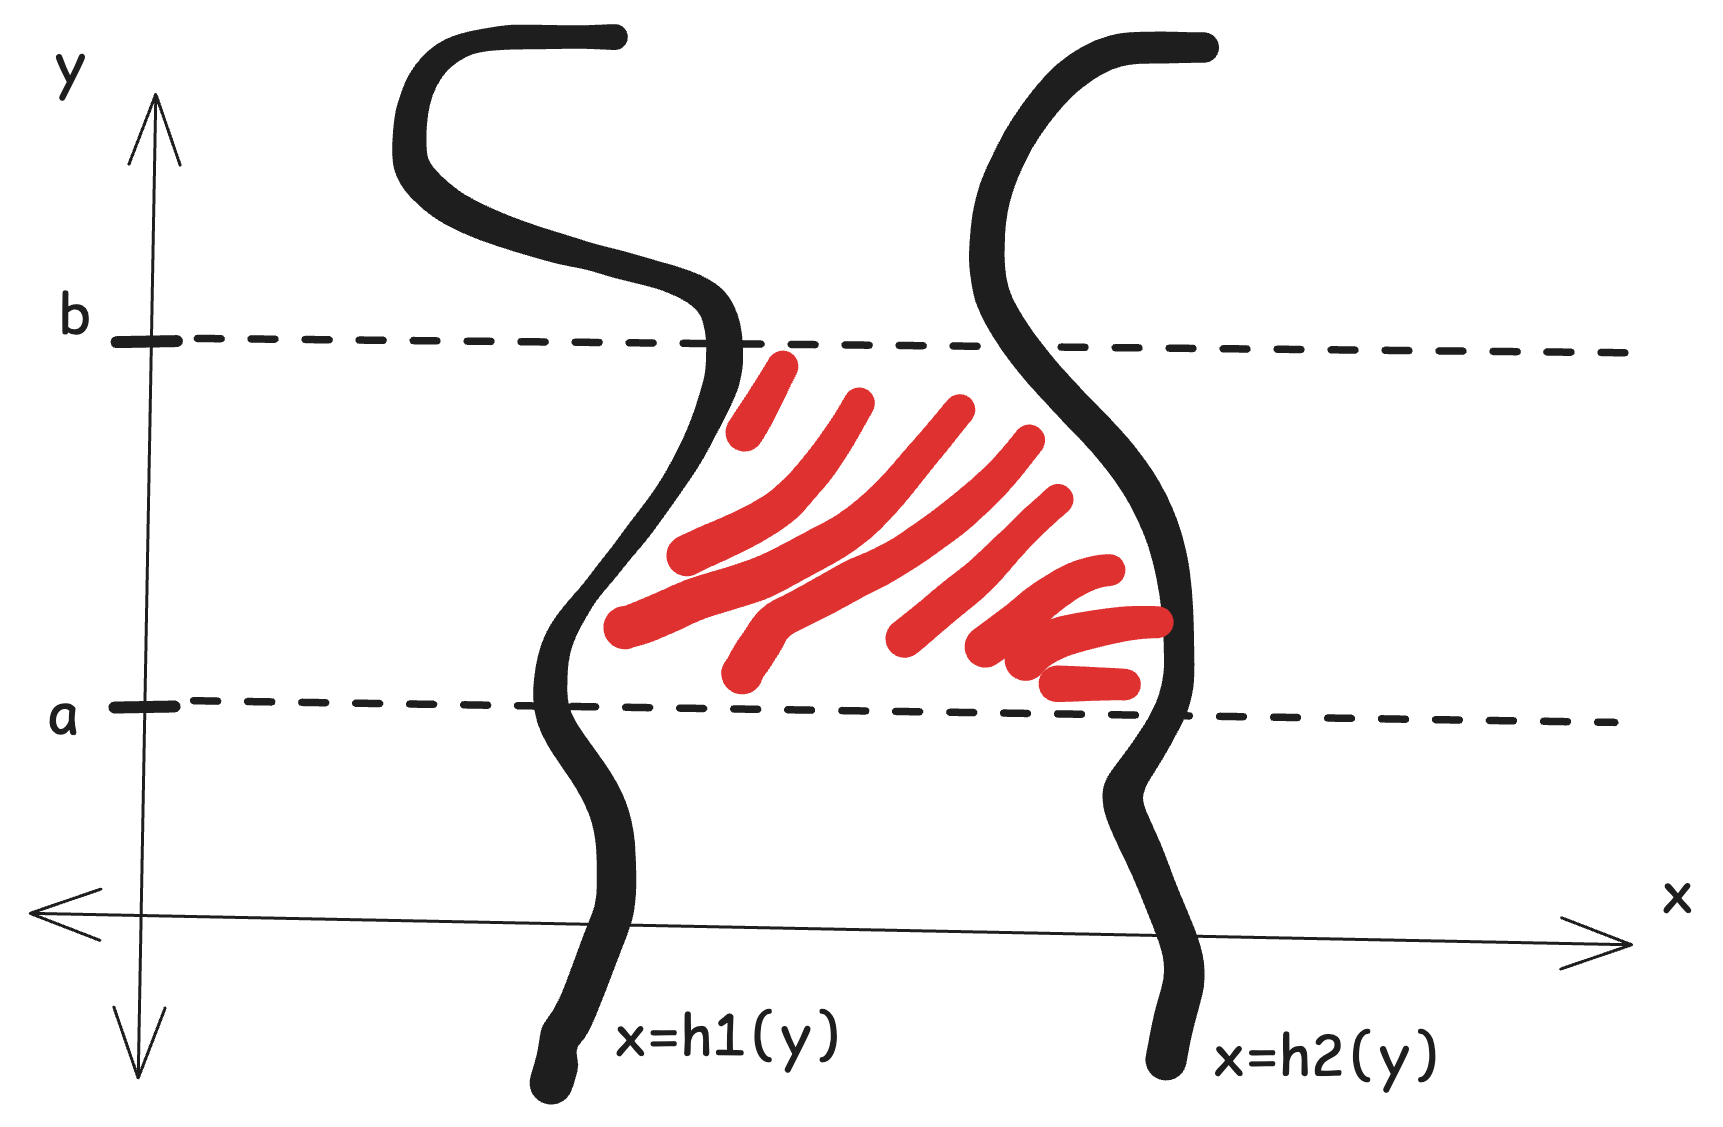
\includegraphics[width=0.5\textwidth]{images/Type2Example.png}
    \caption{Example of a Type 2 Bound}
\end{figure}

\end{document}